\documentclass[../main.tex]{subfiles}
\usepackage{pdfpages}
\begin{document}

\section{Implementación}

\subsection{Preprocesamiento}

Las siguiente páginas pertenecen a la exportación de un archivo \texttt{Jupyter Notebooks} a \texttt{.pdf}.

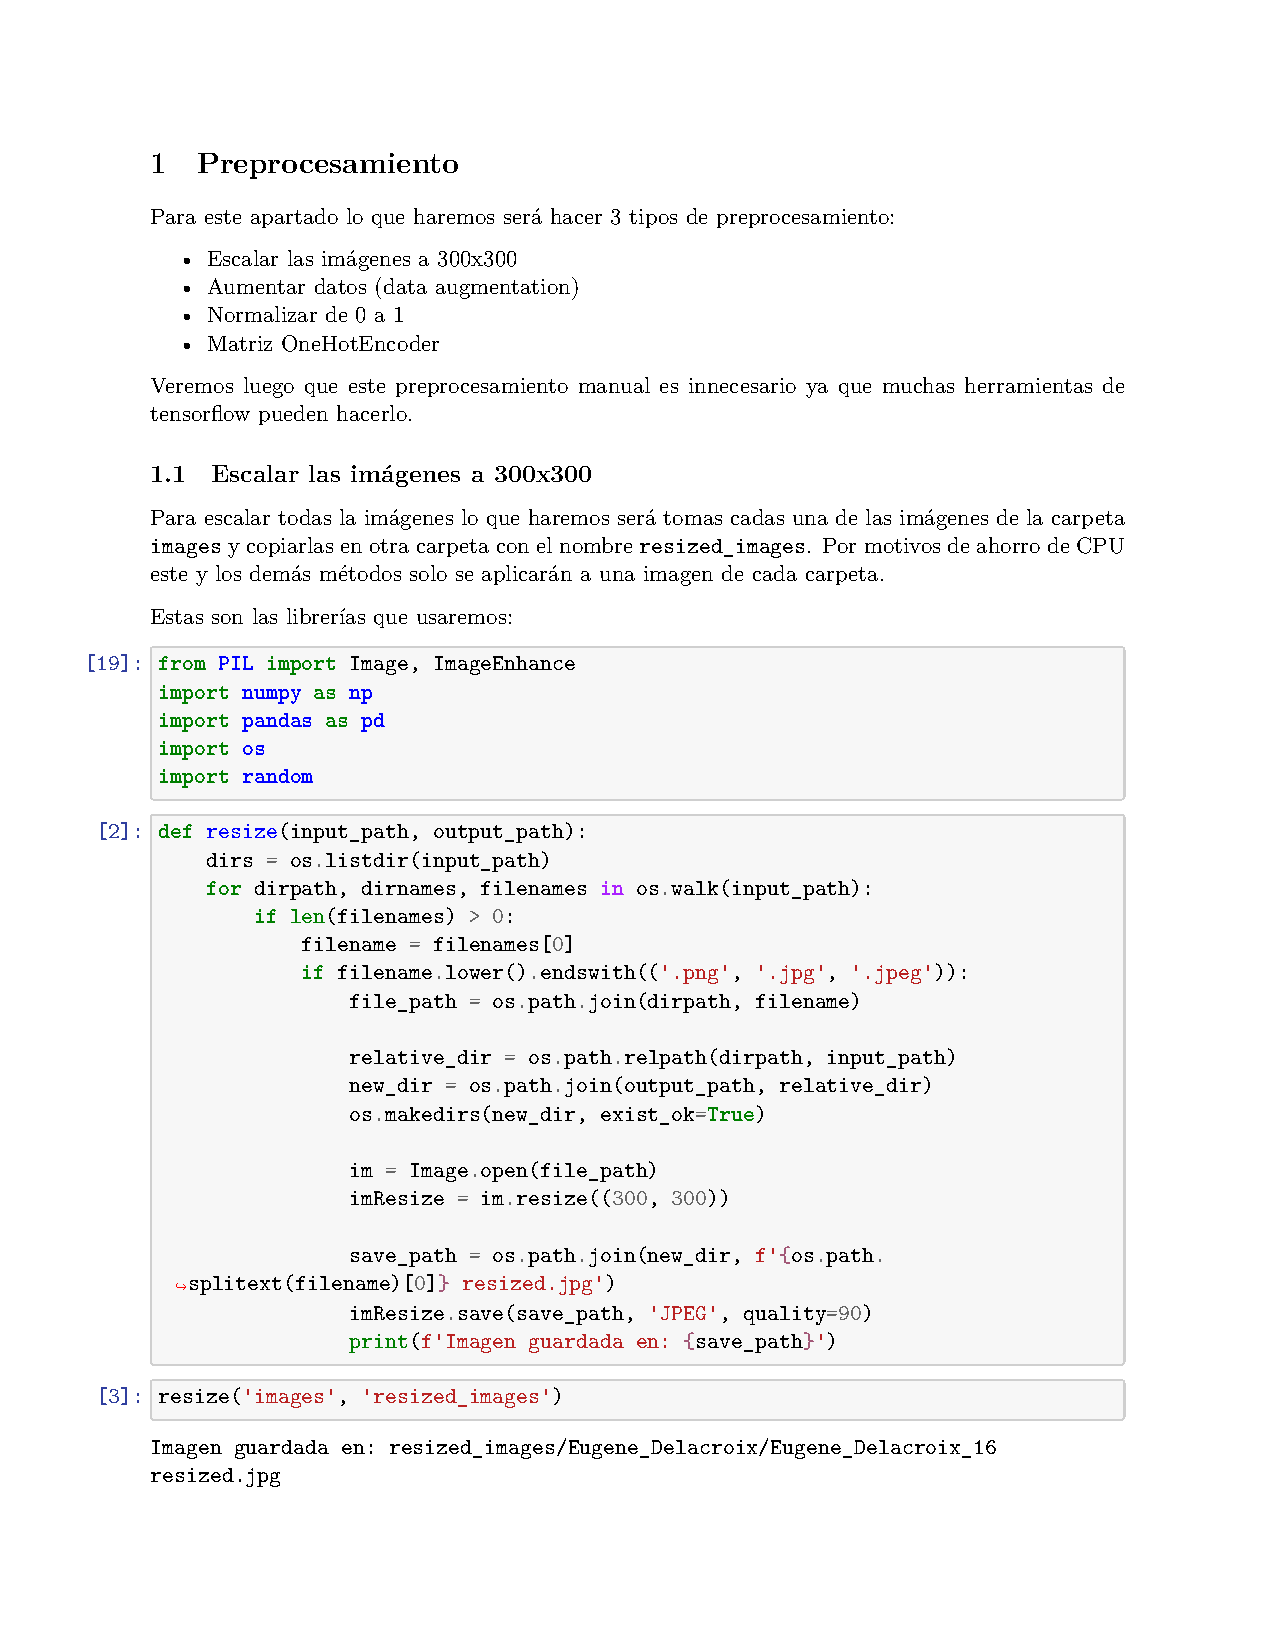
\includepdf[pages=-]{notebooks/preprocesamiento.pdf}

\subsection{Justificación del modelo}

El modelo presentado es un clasificador basado en una red neuronal convolucional (CNN) diseñada para identificar al artista de una pintura. Se basa en el ejemplo del usuario \textbf{mkkoehler} de la plataforma \url{www.kaggle.com} \cite{Mkkoehler_2020} A continuación, se explican las razones detrás de las decisiones de diseño del modelo y su configuración:

\subsubsection{Razones para usar este modelo}

\begin{figure}[htbp] % 'h' posiciona la figura cerca del texto
  \centering
  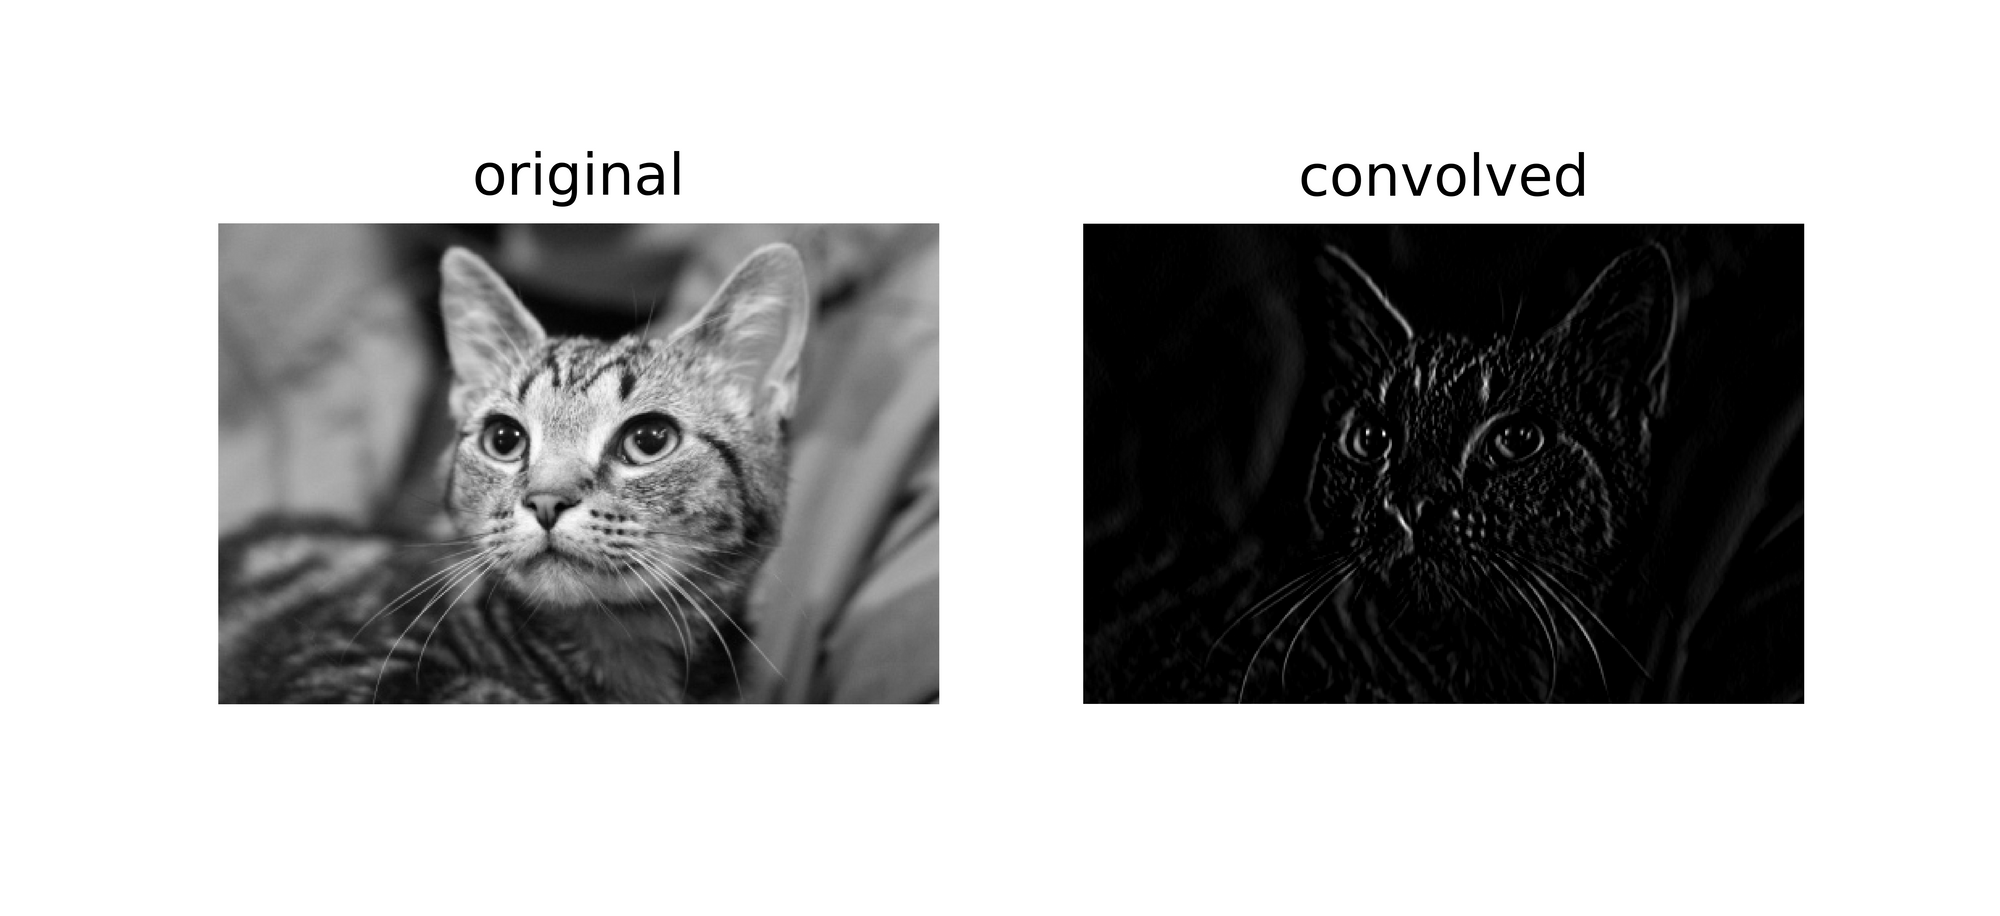
\includegraphics[width=\columnwidth]{convoled_cat} % Ajuste al ancho de la columna
  \caption{Convolución aplicada sobre la imagen de un gato.}
  \label{fig:convoled_cat} % Etiqueta para referencia cruzada
\end{figure}

\begin{itemize}

  \item \textbf{Problema de clasificación de imágenes}:
  
  El problema requiere analizar imágenes para clasificarlas según múltiples categorías (en este caso artistas). Las redes convolucionales son ideales para este propósito debido a su capacidad para detectar patrones espaciales y características visuales en imágenes.

  Como se puede ver en la Figura~\ref{fig:convoled_cat} la convolución actua como un filtro. Gracias a estos filtros es posible que una máquina pueda detectar cosas como los bordes, los colores, las formas, y puede ser que se abstraingan tanto que empieza a ver atributos que nosotros no detectamos, o no podemos nombrar con tanta facilidad, las llamadas características de alto nivel.

  Por ejemeplo, en un paper famosos se uso un dataset de 1.2 millones de imágenes. Sin embargo recuerda que a pesar de los grande logros que tuvo las CNN's en datasets como el MNIST, la implementación para dataset de alta calidad aun son computacionalmente costosas.

  La arquitectura del modelo expuesto en el paper se compone de 8 capas entrenadas, 5 convolucionales, y 3 capas totalmente conectadas. Esta es la arquitectura de AlexNet \cite{krizhevsky2012imagenet}  (Figura~\ref{fig:convoled_cat}). Y de hecho, el número de capas a usar en nuestro modelo como indica el siguiente fragmento, no sigue a unas reglas estrictas, si no más bien que se basan en otras arquitecturas ya probadas.

  \begin{displayquote}
    There are no strict rules on the number of layers which are incorporated in the network model. However, in most cases, two to four layers have been observed in different architectures including LeNet, AlexNet, and VGG Net \cite{alom2018history}
  \end{displayquote}

  Así pues, tomaremos muchas cosas que ya estan en AlexNet como lo son:

  \begin{itemize}
    \item \textbf{Data Augmentation}:

    Aumentar los datos artificialmente aplicando transformaciones que no afecten la escencia de las imágenes, como rotaciones, acercamiento y volteados

    \item \textbf{Scaling}:

    Normalizar los valores de los píxeles de un rango de [0, 255] a [0, 1] para facilitar el entrenamiento del modelo.

    \item \textbf{Primera capa convolucional}:

    La capa convolucional tendra 16 kernels de \(3 \times 3\).

    \item \textbf{Primera capa MaxPooling2D}:

    Esta capa reduce dimensionalidad al seleccionar el valor máximo en regiones específicas, reteniendo la información más importante mientras disminuye la carga computacional.

    \item \textbf{Segunda capa convolucional}:

    La capa convolucional tendra 32 kernels de \(3 \times 3\).

    \item \textbf{Segunda capa MaxPooling2D}

    \item \textbf{Tercera capa convolucional}:
    
    La capa convolucional tendra 64 kernels de \(3 \times 3\).

    \item \textbf{Tercera capa MaxPooling2D}
    
    \item \textbf{Capa Dropout}:
    
    Esta capa apaga el 20\% de las neuronal aleatoriamente. Esto hace que las neuronas sean más robustas a la hora de detectar patrones y también ayuda ayuda a prevenir el sobreajuste

    \item \textbf{Capa de aplanamiento}:
    
    Convierte la salida tridimensional de las capas convolucionales en un vector unidimensional, permitiendo que las capas densas procesen la información.

    \item \textbf{Primera capa densa}
    
    Esta capa se conectará con todas las salidas anteriores, y tendrá 128 neuronas con la función de activación \textbf{ReLu}. Esta recibira cada una de las características que pudo extraer las capas convolucionales.

    \item \textbf{Segunda capa densa, salida}
    
    Esta capa tendrá la misma cantidad de clases como neuronas de salida. Hablamos de 49 clases. Cada neurona se conecta con todas la anterior y se activa cuando la imagen de entrada pertecene a la clase asignada a la neurona. Para esta última capa usaremos las función de activación \textbf{Softmax} para poder ver los porcentajes de salida.

  \end{itemize}

  Entonces nuestro modelo tendrá la siguiente estrucuta:

  \begin{minted}{python}
data_augmentation = keras.Sequential(
  [
    layers.experimental.
    .preprocessing.
      .RandomFlip
      ("horizontal_and_vertical"),
    layers.experimental.
    .preprocessing.
      .RandomRotation(0.25),
    layers.experimental.
    .preprocessing.
      .RandomZoom(0.2), 
    layers.experimental.
    .preprocessing.
      .RandomTranslation(0.3,0.2), 
    layers.experimental.
    .preprocessing.
      .RandomContrast(0.2)
  ]
)
  \end{minted}

  \begin{minted}{python}
CONV = 3

model = Sequential([
  data_augmentation,
  layers.experimental.
   .preprocessing.Rescaling(1./255),
  layers.Conv2D(16, CONV,
                padding='same',
                activation='relu'),
  layers.MaxPooling2D(),
  layers.Conv2D(32, CONV,
                padding='same',
                activation='relu'),
  layers.MaxPooling2D(),
  layers.Conv2D(64, CONV,
                padding='same',
                activation='relu'),
  layers.MaxPooling2D(),
  layers.Dropout(0.2),
  layers.Flatten(),
  layers.Dense(128, activation='relu'),
  layers.Dense(num_classes,
               activation='softmax')
])

  \end{minted}


\begin{figure}[htbp] % 'h' posiciona la figura cerca del texto
  \centering
  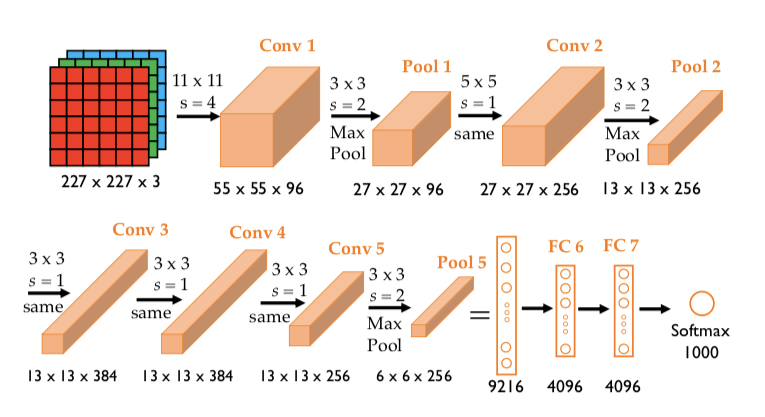
\includegraphics[width=\columnwidth]{alex_net} % Ajuste al ancho de la columna
  \caption{AlexNet. Diagrama de su arquitectura}
  \label{fig:alex_net} % Etiqueta para referencia cruzada
\end{figure}

  \item \textbf{Cantidad de datos}: 
  
  Los datos que usaremos serán de un dataset de \url{www.kaggle.com} explicado en la sección \ref{sec:dataset_explanation}. Con un dataset de 8000 pinturas de más de 49 artistas, un modelo convolucional implementado desde cero es manejable. Sin embargo si se tratara de un dataset con mayor cantidad de datos, lo mejor sería usar modelos ya entrenados.

  En base a el dataset de MNIST \cite{MNIST} que tiene 70.000 imágenes (60.000 para el entrenamiento y 10.000 para la validación) podríamos pensar que nuestro dataset es muy pequeño. Sin embargo hay que tomar en cuenta lo siguiente:

  \begin{enumerate}
    \item Nuestro dataset usa colores RGB.
    \item Usamos data augmentation para poder enriquecer nuestro modelo.
    \item Nuestros recursos computacionales son limitados.
  \end{enumerate}

Por lo tanto, en base a los anteriores podemos proseguir con la exposición.

\end{itemize}

\subsubsection{Elección de las entradas y el tamaño de la imagen}

\begin{itemize}
  \item \textbf{Resolución de entrada (300x300)}: 
  
  Las arquitecturas como AlexNet \cite{krizhevsky2012imagenet} tienen el tamaño de entreada de \(227 \times 227\). Pero como se está trabajando con imágenes de pinturas debemos balancear el tamaño de entrada entre la calidad y la eficiencia. Es por ello que se escogió un tamaño de entrada de \(300 \times 300\) que permite analizar un poco más de detalles sin sacrificar la eficiencia.

  \item \textbf{Tamaño de salida (número de artistas)}:
  
  El modelo finaliza con una capa \texttt{Dense(num\_classes)} donde \texttt{num\_classes} corresponde al número de artistas (49 en nuestro caso) (categorías) Esto permite asignar probabilidades a cada clase durante la clasificación. De hecho este no es el único cámino que existe. Se han intentando otro tipo de codificaciones, como por ejemplo la binaria en el dataset de MNIST \cite{wei2023binary}. En este último estudio revela que tanto la codificación One Hot Encoder como la binaria son igual de eficinetes, sin embargo la codificación binaria es un poco más complicada de decodificar, y por ende de entrenar. Es por ello que por simplicidad por simplicidad usaremos la codificación One Hot Encoder.

\end{itemize}

\subsubsection{Configuración del entrenamiento}

\begin{itemize}
  \item \textbf{Batch size}:
  Este tamaño común en ejemplos de \url{www.kaggle.com} que balancea la estabilidad del gradiente y el uso eficiente de la memoria. Existen sin embargo investigaciones que sugieren un batch size mayor a 200 dependiendo los recursos computacionales \cite{radiuk2017impact}. Sin embargo, dado que nuestros recursos computacionales son limitados (no se cuenta con una GPU) reduciremos el tamaño del lote a 32 que es poco pesado para nuestra computadora, pero funciona.

  \item \textbf{Optimización con RMSprop}:
  El optimizador RMSprop ajusta dinámicamente la tasa de aprendizaje para cada parámetro en función de los gradientes recientes, lo que lo hace particularmente útil en redes neuronales profundas. Su funcionamiento se basa en los siguientes pasos:

  \begin{enumerate}
  \item \textbf{Cálculo del gradiente}:
     \[
     g_t = \nabla_{\theta_t} L(\theta_t)
     \]
     Aquí, \( g_t \) es el gradiente del parámetro \( \theta \) con respecto a la función de pérdida \( L \) en el paso \( t \).
  
  \item \textbf{Promedio móvil del gradiente cuadrado}:
     RMSprop mantiene un promedio exponencial del cuadrado del gradiente:
     \[
     E[g^2]_t = \gamma E[g^2]_{t-1} + (1 - \gamma) g_t^2
     \]
     Donde:
    \begin{itemize}
      \item \( \gamma \): Tasa de decaimiento, típicamente \( \gamma = 0.9 \).
      \item \( E[g^2]_t \): Promedio móvil del gradiente cuadrado en el paso \( t \).
    \end{itemize}
  
  \item \textbf{Actualización del parámetro}:
    La actualización se realiza normalizando el gradiente con la raíz del promedio móvil, añadiendo un término pequeño para evitar divisiones por cero:
    \[
    \theta_{t+1} = \theta_t - \frac{\eta}{\sqrt{E[g^2]_t + \epsilon}} g_t
    \]
    Donde:
    \begin{itemize}
      \item \( \eta \): Tasa de aprendizaje.
      \item \( \epsilon \): Término de estabilidad numérica, típicamente \( \epsilon = 10^{-8} \).
    \end{itemize}

  \end{enumerate}
  
  Lo que hace a grandes rasgos cada una de las ecuaciones es:
  
  \begin{enumerate}
  \item \textbf{Promedio móvil del gradiente cuadrado}:  
     El término \( E[g^2]_t \) acumula la información histórica del gradiente, permitiendo que RMSprop adapte la escala de las actualizaciones de los parámetros basándose en la magnitud del gradiente reciente.
  
  \item \textbf{Normalización adaptativa}:  
     Al dividir por \( \sqrt{E[g^2]_t + \epsilon} \), RMSprop reduce la magnitud de las actualizaciones en parámetros con gradientes grandes y las aumenta en parámetros con gradientes pequeños. Esto permite que el modelo aprenda de manera más uniforme y evita que los gradientes grandes dominen el entrenamiento.
  
  \item \textbf{Tasa de aprendizaje efectiva}:  
     En cada paso, RMSprop calcula una tasa de aprendizaje efectiva específica para cada parámetro, adaptándola según el historial de gradientes.
  \end{enumerate}

  El código que inicializa este optimizador es:

  \begin{minted}{python}
opti = tf.keras.optimizers.
 .RMSprop(momentum=0.1) 
  \end{minted}

  Aunque el parámetro momentum no aparece explícitamente en las ecuaciones de \textbf{RMSprop}, se incluye en la implementación de TensorFlow para mantener una interfaz unificada con otros optimizadores y para que el optimizador no se quede atrapado en mínimos locales. Existen más parámetros que se pueden especificar según la página de Keras. Además en la misma página nos dice el valor por defecto de la tasa de aprendizaje.

  
  \begin{displayquote}
    \begin{itemize}
      \item \textbf{momentum}: \texttt{float}, defaults to 0.0. If not 0.0., the optimizer tracks the momentum value, with a decay rate equals to 1 - momentum.
      \item \textbf{learning\_rate}:
      A \texttt{float}, a \texttt{keras. optimizers. schedules. LearningRateSchedule} instance, or a callable that takes no arguments and returns the actual value to use. The learning rate. Defaults to 0.001. \cite{keras_rmsprop}
    \end{itemize}
  \end{displayquote}

  

  \item \textbf{Pérdida (SparseCategoricalCrossentropy)}: 
  La pérdida \textbf{SparseCategoricalCrossentropy} se utiliza para problemas de clasificación multiclase donde las etiquetas de las clases son enteros (en lugar de vectores one-hot). Es especialmente útil cuando hay un número grande de clases, ya que reduce los requisitos de memoria y cómputo. Esta tiene una relación estrecha con la función de entropía cruzada estándar está definida como:

  \[
  L_{\text{CCE}} = -\frac{1}{N} \sum_{k=1}^{N} \sum_{i=1}^{C} y_{k,i} \log(\hat{y}_{k,i})
  \]

  Donde:

  \begin{itemize}
      \item \(N\): Número de ejemplos en el lote.
      \item \(C\): Número de clases.
      \item \(y_{k,i}\): Valor de la etiqueta para el ejemplo \(k\) y la clase \(i\) (one-hot-encoded: \(1\) para la clase correcta, \(0\) para las demás).
      \item \(\hat{y}_{k,i}\): Probabilidad predicha para el ejemplo \(k\) y la clase \(i\).
  \end{itemize}

  En el caso de \textbf{SparseCategoricalCrossentropy}, no se utiliza un vector codificado one-hot (\(y_{k,i}\)), sino un entero \(t_k\) que representa el índice de la clase correcta para el ejemplo \(k\). La fórmula se simplifica:

  \[
  L_{\text{SparseCCE}} = -\frac{1}{N} \sum_{k=1}^{N} \log(\hat{y}_{k,t_k})
  \]

  Donde:

  \begin{itemize}
      \item \(t_k\): Índice entero de la clase correcta para el ejemplo \(k\).
      \item \(\hat{y}_{k,t_k}\): Probabilidad predicha para la clase \(t_k\).
  \end{itemize}

  Así pues, ambas funciones son equivalentes si las etiquetas \(t_k\) se convierten en formato one-hot. La diferencia es puramente en términos de representación y eficiencia computacional.

  \[
  L_{\text{CCE}} = L_{\text{SparseCCE}}
  \]

  La distinción surge porque en \textbf{SparseCategoricalCrossentropy}, en lugar de sumar sobre todas las clases \(i\), simplemente se accede directamente al valor de la probabilidad predicha para la clase correcta, \(t_k\).

  Esta pérdida generalmente se usa junto con una activación \textbf{ softmax} en la última capa de la red neuronal. El softmax convierte las salidas \(z_i\) del modelo en probabilidades \(\hat{y}_i\):

  \[
  \hat{y}_i = \frac{e^{z_i}}{\sum_{j=1}^{C} e^{z_j}}
  \]

  Donde:

  \begin{itemize}
      \item \(z_i\): Logits o puntuaciones brutas producidas por el modelo para la clase \(i\).
      \item \(C\): Número total de clases.
  \end{itemize}

  La combinación de softmax y entropía cruzada es eficiente, ya que se pueden calcular juntos de manera numéricamente estable mediante la opción \texttt{from\_logits=True}.

  En TensorFlow el código es:

  \begin{minted}{python}
loss = tf.keras.losses.
 .SparseCategoricalCrossentropy
  (from_logits=True) 
  \end{minted}

  \item \textbf{Medida de precisión}:
   
  El \textbf{accuracy} o \textbf{precisión} es una métrica de evaluación utilizada en problemas de clasificación que mide la proporción de predicciones correctas respecto al total de predicciones. Matemáticamente, se define como:

  \[
  \text{Accuracy} = \frac{\text{Número de predicciones correctas}}{\text{Número total de predicciones}}
  \]

  La fórmula matemática es:

  Dado un conjunto de datos con \( N \) muestras:

  \begin{enumerate}
      \item \( y_{\text{true}} \): etiquetas reales de las muestras.
      \item \( y_{\text{pred}} \): etiquetas predichas por el modelo.
  \end{enumerate}

  La precisión se calcula como:
  \[
  \text{Accuracy} = \frac{\sum_{i=1}^{N} \delta(y_{\text{pred}_i} = y_{\text{true}_i})}{N}
  \]
  donde
  :
  \[
  \delta(y_{\text{pred}_i}, y_{\text{true}_i}) = 
  \begin{cases} 
    1 & \text{si } y_{\text{pred}_i} = y_{\text{true}_i}, \\
    0 & \text{en caso contrario.}
  \end{cases}
  \]

  En TensorFlow, la métrica \texttt{accuracy} realiza internamente este cálculo utilizando las predicciones del modelo y las etiquetas reales. En este caso:

  \begin{enumerate}
      \item El modelo produce un vector de probabilidades (logits) por clase, ya que se usa \texttt{SparseCategoricalCrossentropy (from\_logits=True)}.
      \item \texttt{'accuracy'} convierte los logits en índices de clases predichas (aplicando \texttt{argmax} en el eje de las clases).
      \item Compara estas predicciones con las etiquetas reales para calcular la fracción de aciertos.
  \end{enumerate}

  El \texttt{accuracy} es una métrica adecuada cuando:

  \begin{itemize}
      \item Las clases están balanceadas (aproximadamente el mismo número de muestras por clase).
      \item La evaluación del modelo no necesita diferenciar entre tipos de errores (por ejemplo, en problemas médicos donde los falsos negativos pueden ser más graves que los falsos positivos).

  \end{itemize}

  \item \textbf{Épocas}:
  
  Empezaremos con 20 épocas (ya que el ejemplo viene definido así). Si es que el modelo no convergiera, entonces se podría modificar levemente algunos de los hiperparámetros. Si es que si convergiera entonces lo que procedería es aumentar el número de épocas. En una primera ejecución se pudo evidenciar que el modelo podía distinguir algunas pinturas, sin embargo, no era tan preciso commo se esperaría.

  \item \textbf{Entrenamiento}
  
  Cuando usamos el método \texttt{model.fit} lo que TensorFlow hace es:
  \begin{enumerate}
      \item \textbf{Forward Pass (Propagación hacia adelante)}:
      \begin{itemize}
          \item La imagen pasa a través de las capas convolucionales (\texttt{Conv2D}), donde los kernels realizan convoluciones, detectando características como bordes o texturas.
          \item Luego, las capas densas combinan estas características para hacer predicciones.
          \item Finalmente, el modelo genera una salida con probabilidades para cada clase, gracias a la capa \texttt{Dense} con activación \texttt{softmax}.
      \end{itemize}

      Matemáticamente:

      \begin{enumerate}
          \item Para cada capa convolucional (\texttt{Conv2D}):
          \[
          \mathbf{y}^{(l)} = \text{ReLU}\left(\mathbf{W}^{(l)} * \mathbf{x}^{(l-1)} + \mathbf{b}^{(l)}\right)
          \]
          donde:
          \begin{itemize}
              \item \(\mathbf{W}^{(l)}\) son los filtros o kernels de la capa \(l\).
              \item \(*\) denota la operación de convolución.
              \item \(\mathbf{x}^{(l-1)}\) es la salida de la capa anterior.
              \item \(\mathbf{b}^{(l)}\) son los sesgos de la capa.
              \item \(\text{ReLU}(z) = \max(0, z)\) es la función de activación.
          \end{itemize}
          \item Las capas densas (\texttt{Dense}) combinan las características extraídas:
          \[
          \mathbf{y}^{(L)} = \text{ReLU}\left(\mathbf{W}^{(L)} \cdot \mathbf{x}^{(L-1)} + \mathbf{b}^{(L)}\right)
          \]
          donde:
          \begin{itemize}
              \item \(\cdot\) denota el producto matricial,
              \item \(\mathbf{W}^{(L)}\) son los pesos de la capa \(L\),
              \item \(\mathbf{x}^{(L-1)}\) es la salida de la capa anterior.
          \end{itemize}
          \item La capa final usa \texttt{softmax} para generar probabilidades para cada clase:
          \[
          \hat{y}_i = \frac{\exp(z_i)}{\sum_{j} \exp(z_j)}
          \]
          \[
          \text{para cada } i = 1, \dots, \text{num\_classes}
          \]
          donde:
          \begin{itemize}
              \item \(z_i\) es la entrada a la clase \(i\),
              \item \(\hat{y}_i\) es la probabilidad predicha para la clase \(i\).
          \end{itemize}
      \end{enumerate}

      \item \textbf{Cálculo del error}:

      El modelo compara las predicciones con las etiquetas reales usando la función de pérdida (\texttt{SparseCategoricalCrossentropy} en este caso). Esto genera un valor de pérdida que indica qué tan incorrecta fue la predicción.


      \item \textbf{Backward Pass (Propagación hacia atrás)}:

      \begin{itemize}
          \item Se usa el algoritmo de \textbf{backpropagation} para calcular el gradiente de la pérdida con respecto a todos los parámetros entrenables (pesos de las capas densas y kernels de las convoluciones).
          \item El optimizador (\texttt{RMSprop}) actualiza los valores de los parámetros para minimizar la pérdida.
          \begin{enumerate}
              \item Calcula los gradientes para cada parámetro.
              \item Actualiza los valores de los parámetros en base al gradiente y su hiperparámetro de aprendizaje.
          \end{enumerate}
      \end{itemize}

      Matemáticamente:

      \begin{enumerate}
          \item \textbf{Gradientes}:
          Se calculan los gradientes de la pérdida con respecto a los parámetros entrenables (\(\mathbf{W}\) y \(\mathbf{b}\)):
          \begin{itemize}
              \item Para los pesos de la capa \(l\):
              \[
              \frac{\partial \mathcal{L}}{\partial \mathbf{W}^{(l)}} = \mathbf{\delta}^{(l)} \cdot (\mathbf{x}^{(l-1)})^\top
              \]
              \item Para los sesgos de la capa \(l\):
              \[
              \frac{\partial \mathcal{L}}{\partial \mathbf{b}^{(l)}} = \mathbf{\delta}^{(l)}
              \]
              \item Donde \(\mathbf{\delta}^{(l)}\) es el gradiente del error propagado hacia atrás en la capa \(l\), calculado como:
              \[
              \mathbf{\delta}^{(l)} = \frac{\partial \mathcal{L}}{\partial \mathbf{y}^{(l)}} \cdot f'(\mathbf{z}^{(l)})
              \]
          \end{itemize}
          \item \textbf{Actualización de parámetros}:
          Los gradientes se utilizan para actualizar los parámetros con un optimizador (\texttt{RMSprop} en este caso). Usando la regla de descenso de gradiente:
          \[
          \mathbf{W}^{(l)} \leftarrow \mathbf{W}^{(l)} - \eta \cdot \frac{\partial \mathcal{L}}{\partial \mathbf{W}^{(l)}}
          \]
          \[
          \mathbf{b}^{(l)} \leftarrow \mathbf{b}^{(l)} - \eta \cdot \frac{\partial \mathcal{L}}{\partial \mathbf{b}^{(l)}}
          \]
          donde \(\eta\) es la tasa de aprendizaje.
      \end{enumerate}

    \end{enumerate}

  Los parámetros que se actualizan son:

  \begin{enumerate}
      \item Kernels en las capas convolucionales (\texttt{Conv2D})
      \(\mathbf{W}^{(l)}\) y \(\mathbf{b}^{(l)}\)
      \item Pesos y sesgos en las capas densas (\texttt{Dense})
      \(\mathbf{W}^{(L)}\) y \(\mathbf{b}^{(L)}\)
  \end{enumerate}

  Así hay algunas cosas que cabe señalar como:

  \begin{enumerate}
    \item TensorFlow permite que nosotros hagamos modificaciones a el método  \texttt{fit()} creando una clase que herede de nuestro modelo y sobre escribiendo el método \texttt{train\_step()} \cite{customizing_fit}
    \item Del mismo modo TensorFlow permite poder hacer nuestros propios layers totalmente personalizados, inclusive con pesos no entrenables \cite{making_new_layer}
  \end{enumerate}

\end{itemize}

\end{document}
